\section{Cel i zakres pracy}
Celem pracy było zbudowanie mobilnego robota, który może być wykorzystany do monitorowania budynku.
Podstawowym jego wyposażeniem jest kamera.
Robot jest zdolny do poruszania się na kołach.

Obsługa odbywa się przez aplikację webową (przeglądarkową).
Oprogramowanie pozwala na zdalne sterowanie pojazdem bez kontaktu wzrokowego dzięki strumieniowaniu obrazu z kamery na żywo.
Dane wizualne z kamery są gromadzone i regularnie wysyłane na zdalny nośnik.
Aplikacja jest zabezpieczona przed nieupoważnionymi osobami i pozwala na zarządzanie dostępem użytkowników.

\section{Problematyka}
Monitoring miejsc, obiektów itp. to powszechna praktyka w miejscach zarówno publicznych, jak i prywatnych.
Jest to jeden ze środków ochrony ludzi i mienia.
Jak opisuje artykuł\cite{surveillance_911} opublikowany w \textit{Wall Street Journal}, masowy monitoring prędko się upowszechnił po traumatycznej tragedii zamachu na wieże World Trade Center 11 września 2001 roku.
Obecnie przemysł nadzorowania za pomocą kamer jest wyceniany na ok. 74 miliardy USD\cite{rynek_monitoring} i przewiduje się roczny wzrost na poziomie 12\%.

Ogląd na stan obecny i kierunek rozwoju systemów do wideo monitoringu przedstawiają artykuły naukowe: \cite{surv_review_1} oraz \cite{surv_review_2}.
Najbardziej powszechnym systemem monitoringu jest sieć zainstalowanych na stałe kamer.
Kiedyś były to zamknięte obwody, do których obserwowania trzeba było stale zatrudniać ochroniarzy.
Dziś powszechne są tzw. kamery IP ze stałym podłączeniem do internetu, coraz częściej bezprzewodowym.
Otwiera to drogi do nowych możliwości w zakresie archiwizacji, przetwarzania i podejmowania decyzji na podstawie danych wideo.
Coraz częściej sięga się po zaawansowane metody przetwarzania obrazu wykorzystujące uczenie maszynowe, sztuczną inteligencję.
Stawia się też na zastosowanie szerokiej gamy sensorów oprócz samych kamer.

Jednym z innowacyjnych rozwiązań dotyczących monitoringu są mobilne roboty.
Nie jest to (jeszcze) podejście głównego nurtu, ale pojawiają się głosy mówiące o potrzebie takich rozwiązań, jak i same konstrukcji.
Zaletami takich rozwiązań są m.in.
\begin{itemize}
    \item zwiększenie obszaru pokrytego monitoringiem -- statycznie zamontowane kamery mają martwe pola,
    \item zmniejszenie zasobów potrzebnych na nadzór dużych powierzchni -- wiele kamer statycznych może zastąpić jeden mobilny robot.
\end{itemize}

Na konferencji \textit{2010 IEEE Workshop on Advanced Robotics and its Social Impacts} tematem jednego z wystąpień było \textit{Intelligent surveillance and security robot systems}\cite{5679624}.
Zaprezentowanych zostało kilka typów nowatorskich, inteligentnych rozwiązań do monitoringu, oto opis jednego z nich:

\blockquote{A mobile patrol robot named ‘STAR’, with a unique single pivot design, is driven by four independently steered wheels, which enables changing the direction on the spot.
The mobile robot is designed for surveillance over a vast range of fields with the guidance by a GPS sensor and a scanning laser range finder.}

Ta praca wpisuje się w dziedzinę podobnych rozwiązań.

\section{Powiązane publikacje naukowe}
Przeszukując literaturę naukową w tematyce mobilnych robotów nadzorujących, można zauważyć, że nie jest to popularna dziedzina i wiele prac przedstawia jedynie projekty i/lub niezbyt mocno rozwinięte prototypy.
Tutaj pokrótce przedstawię kilka z ciekawszych pomysłów.

W \cite{shin2016design} opisany jest prototyp jeżdżącego robota wyposażonego w kamerę opartego o platformy Raspberry Pi i Arduino.
Jego oprogramowanie pozwala na sterowanie poprzez stronę internetową, jak i na automatyczne wykrywanie nieprawidłowości w nadzorowanym otoczeniu za pomocą algorytmów analizy obrazu.

Inna konstrukcja tego typu została opisana w \cite{MEDDEB2023104728}.
Robot oparty jest o popularny mikrokomputer Raspberry Pi 4, który steruje silnikami i przetwarza dane z sensorów -- czujnika ruchu PIR i kamery.
Jedną z funkcjonalności jest wykrywanie twarzy i wysyłanie powiadomień o wykryciu nieznanych osób.

W \cite{9375666} przedstawiony jest jeżdżący robot z kamerą, oparty na Raspberry Pi i na mikrokontrolerze Arduino.
Ma on funkcję autonomicznego patrolowania terenu wraz ze zdolnością do omijania przeszkód dzięki zamontowanym czujnikom odległości.

\section{Istniejące rozwiązania komercyjne}
Mimo, że obszar mobilnych robotów nadzorujących może się wydawać nierozwinięty i niedojrzały, to na rynku istnieje kilka firm, których działalność opiera się na tego typu rozwiązaniach.

\label{smp_robot}
Jedną z nich jest \href{https://smprobotics.com/}{SMP Robotics}.
Jej flagową linią produktów są mobilne roboty przeznaczone do nadzoru terenów zewnętrznych.
Są to pojazdy wyposażone w kamerę zamontowaną na słupku, przykładowy model przedstawiony na zdjęciu \ref{rys:smp_robot}.
\begin{figure}[!hb]
    \centering 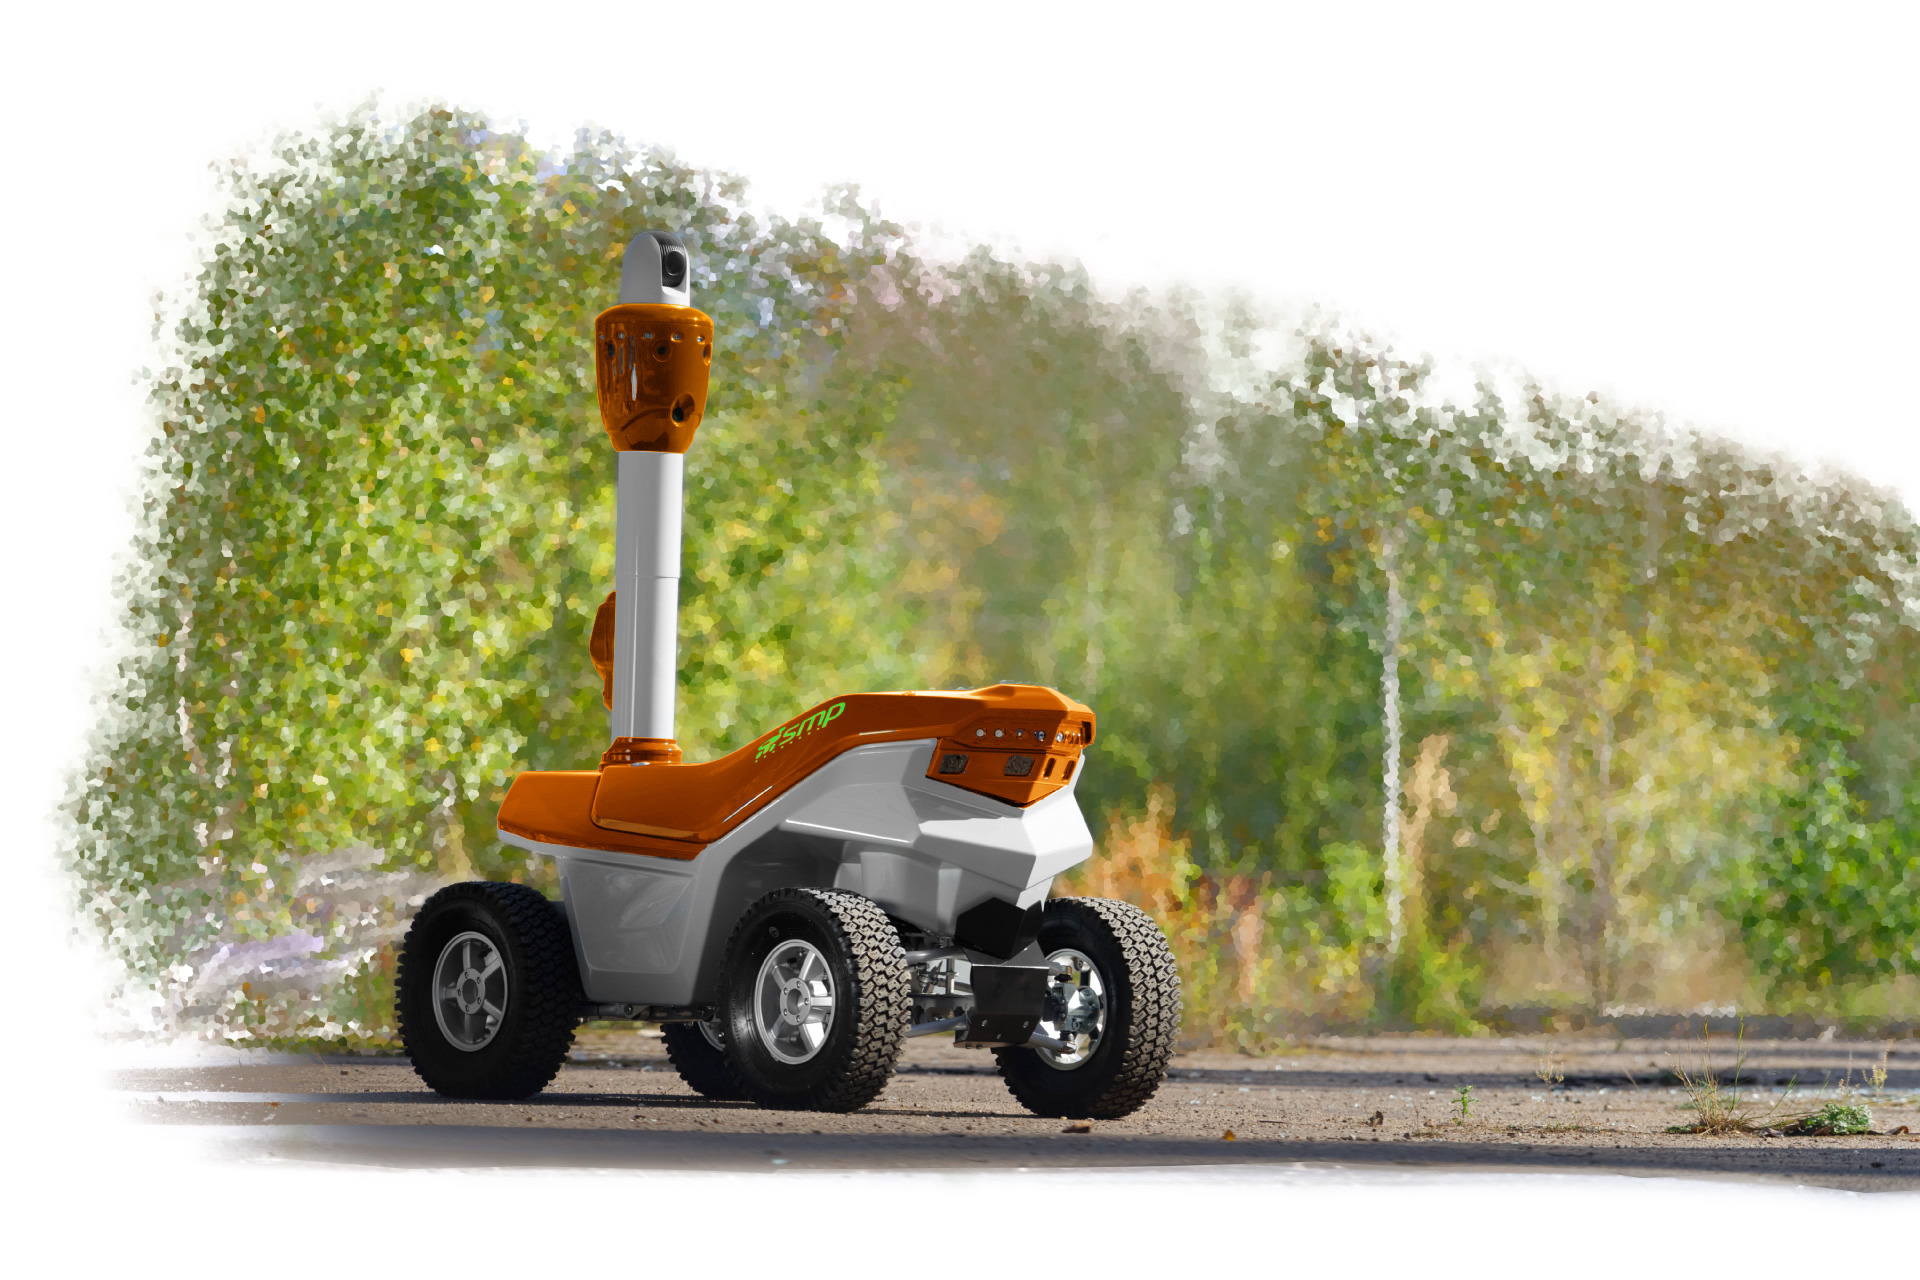
\includegraphics[width=0.618\linewidth]{security_robot_smp.jpg}
    \caption{Robot patrolowy firmy SMP Robotics}
    \label{rys:smp_robot}
\end{figure}
Oferują m.in.: w pełni autonomiczny patrol, sterowanie głosowe, rozpoznawanie twarzy w odległości do 50 metrów i system automatycznego ładowania akumulatorów.

Firma \href{https://robotnik.eu/}{Robotnik} produkuje roboty do różnych zastosowań, w tym model \href{https://robotnik.eu/products/mobile-robots/rb-watcher/}{\textit{RB-Watcher}}.
Jest on przeznaczony do autonomicznego nadzoru wewnątrz budynków, jak i na zewnątrz.
Jego wyposażenie obejmuje bispektralną kamerę, GPS i mikrofon.
Do orientacji w przestrzeni wykorzystuje algorytmy typu SLAM (\textit{Simultaneous localization and mapping}).
Budową przypomina on wspomnianego wyżej robota \ref{smp_robot} od SMP Robotics, ale jest wyraźnie niższy.
Jest on przedstawiony na zdjęciu \ref{rys:robotnik}.
\begin{figure}[!hb]
    \centering 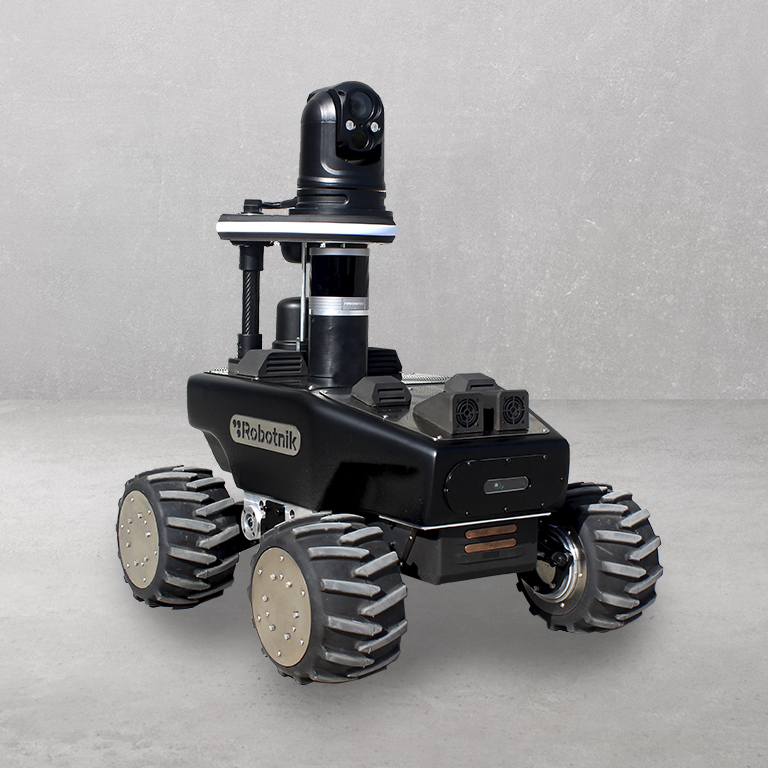
\includegraphics[width=0.618\linewidth]{robotnik.jpg}
    \caption{Robot patrolowy \textit{RB Watcher} firmy Robotnik}
    \label{rys:robotnik}
\end{figure}

Podobne rozwiązanie oferuje firma \href{https://www.knightscope.com/}{Knightscope}.
Na \href{https://www.knightscope.com/products/k5}{stronie internetowej produktu} chwalą się rezultatami zastosowania w postaci:
\begin{itemize}
    \item zmniejszenia liczby zgłaszanych przestępstw o 46\%,
    \item zwiększenia liczby aresztów o 27\%,
    \item zmniejszenia liczby wystawionych mandatów o 68\%.
\end{itemize}
Robot firmy Knightscope wygląda inaczej od przedstawionych wcześniej konkurencyjnych produktów -- widać to na zdjęciu~\ref{rys:knightscope}.
\begin{figure}[!hb]
    \centering 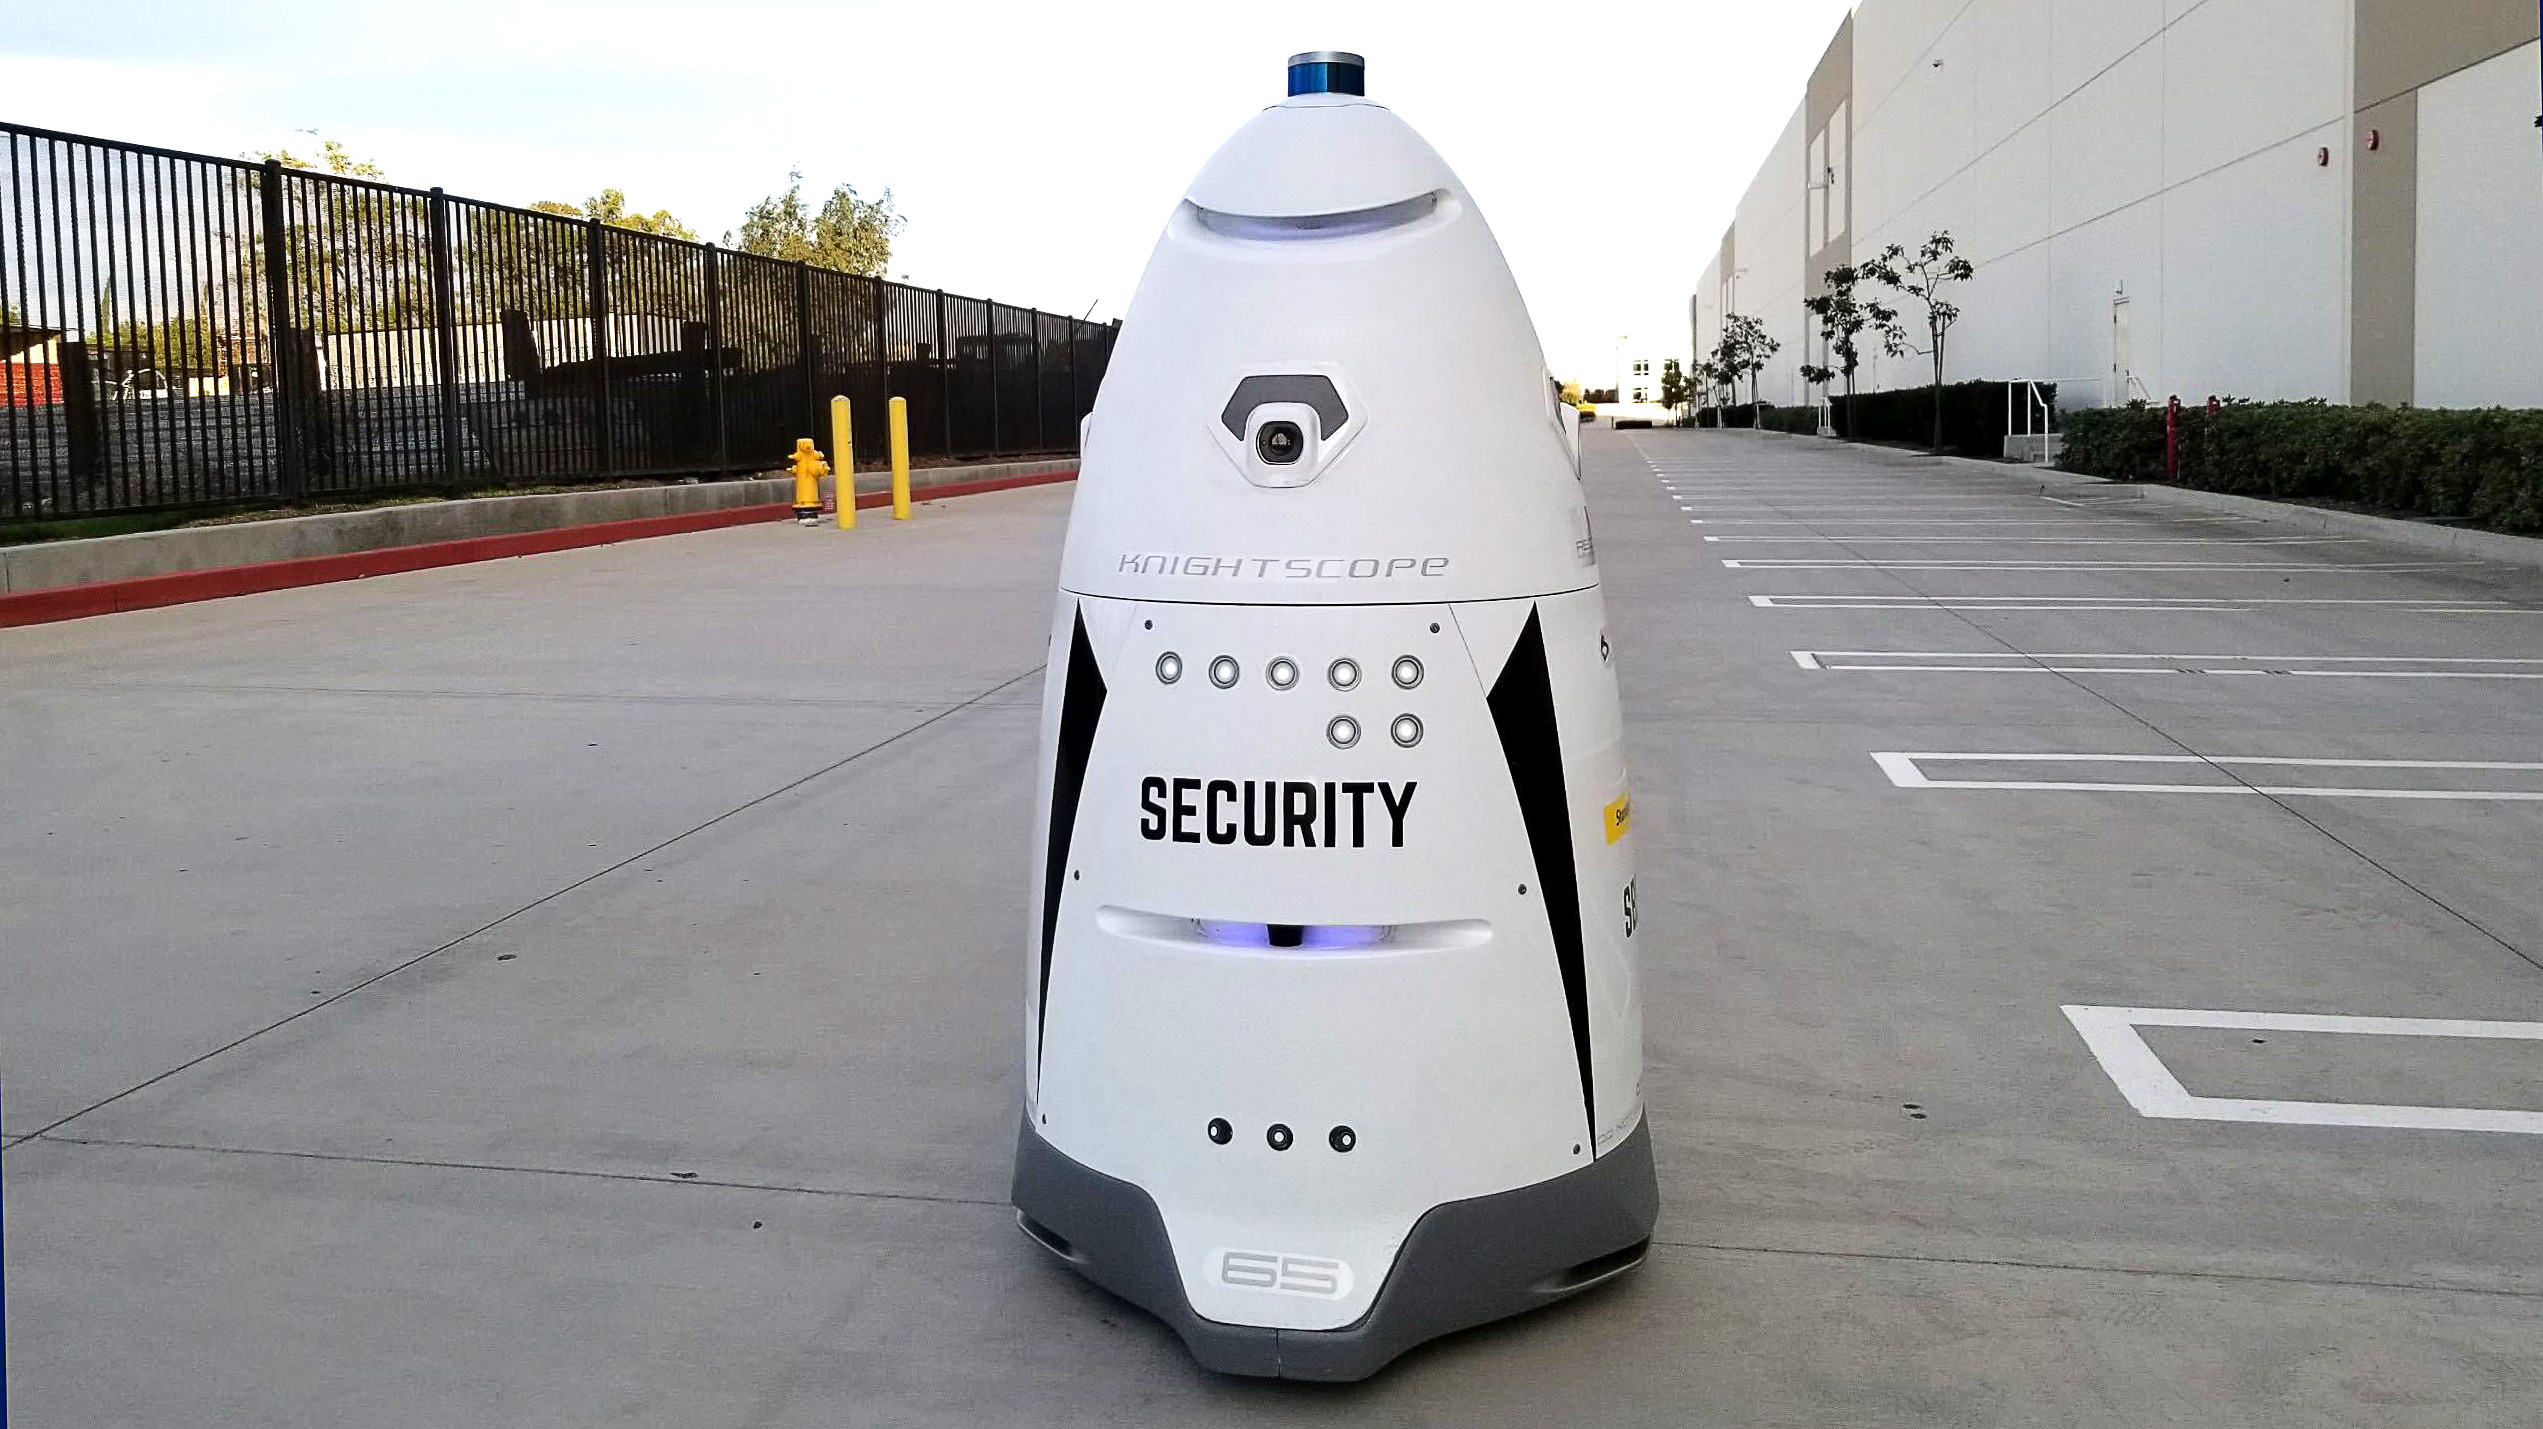
\includegraphics[width=0.618\linewidth]{knightscope.jpg}
    \caption{Robot patrolowy \textit{K5} firmy Knightscope}
    \label{rys:knightscope}
\end{figure}

Mobilne roboty nadzorujące oferują także firmy: Cobalt AI, Running Brains Robotics, Super Droid Robots i inne.

\section{Motywacja}
Obszar mobilnych robotów sprawujących nadzór wydaje się mieć duży potencjał.
Jednocześnie rozwiązania z tej dziedziny nie należą do kanonu narzędzi typowo stosowanych do monitoringu.
Dlatego jest to nisza, która pozostawia w mojej opinii nadal pole do eksploracji.

Zakres tej pracy jest ciekawy ze względu na konieczną fuzję kilku dziedzin inżynierii -- informatyki, elektroniki i mechaniki.
Jako że jednak moją specjalizacją jest informatyka, to najbardziej skupiam się na części związanej z oprogramowaniem robota.
W tym obszarze widzę kilka wyzwań związanych z:
\begin{itemize}
    \item cyberbezpieczeństwem -- zabezpieczenie dostępu do aplikacji webowej, danych użytkowników,
    \item przetwarzaniem danych w czasie rzeczywistym -- przy sterowaniu robotem,
    \item przetwarzaniem multimediów -- strumieniowanie obrazu z kamery do wielu użytkowników.
\end{itemize}
Wyzwania te czynią tę pracę okazją do rozwoju.